% begin module continuity-ex1
\begin{frame}
\begin{example}
The picture below shows a graph of a function $f$.  \alertNoH{2-3}{At which numbers is $f$ either discontinuous or not defined?}  \alertNoH{4-}{Why?}
\begin{columns}[c]
\column{.5\textwidth}
\begin{pspicture}(-0.5, -1.5)(5,5.2) \psframe*[linecolor=white](-0.5,-1)(5,5.2)
\psaxes[ticks=x, labels=x]{<->}(0,0)(-0.5,-0.5)(5,5)
\psplot[linecolor=red, plotpoints=1000]{2}{5}{x 4 exp -0.0454545 mul x 3 exp 0.0555556 mul add x -1 mul add x 2 exp add 0.5 add }
\psplot[linecolor=red, plotpoints=1000]{-0.5}{2}{x 2 exp x 3 exp -0.5 mul add 1 add }
\fcHollowDot{1}{1.5}
\fcFullDot{2}{1}
\fcHollowDot{2}{2.217171717}
\fcHollowDot{4}{4.419191919}
\fcFullDot{4}{2}
\end{pspicture}
%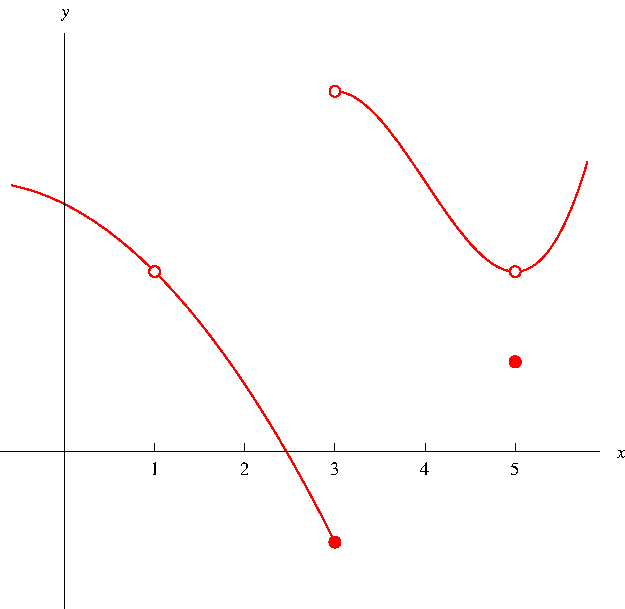
\includegraphics[height=4.5cm]{continuity/pictures/02-05-ex1.pdf}%

\column{.5\textwidth}
\begin{itemize}
\item<3->  Not defined at $1$:
\item<4->  \alertNoH{5-6}{$\lim\limits_{x\rightarrow 1}f(x)$ \fcAnswer{6}{exists.}}
\item<4->  \alertNoH{7-8}{$f(1)$ \fcAnswer{8}{is not defined.}}
\item<3->  Discontinuous at $2$:
\item<4->  \alertNoH{9-10}{$f(2)$ \fcAnswer{10}{is defined.}}
\item<4->  \alertNoH{11-12}{$\lim\limits_{x\rightarrow 2}f(x)$ \fcAnswer{12}{doesn't exist.}}
\item<3->  Discontinuous at $4$:
\item<4->  \alertNoH{13-14}{$f(4)$ \fcAnswer{14}{is defined.}}
\item<4->  \alertNoH{15-16}{$\lim\limits_{x\rightarrow 4}f(x)$ \fcAnswer{16}{exists.}}
\item<17-| alert@17>  $\lim\limits_{x\rightarrow 4}f(x) \neq f(4)$.
\end{itemize}
\end{columns}
\end{example}
\end{frame}
% end module continuity-ex1
